
%(BEGIN_QUESTION)
% Copyright 2007, Tony R. Kuphaldt, released under the Creative Commons Attribution License (v 1.0)
% This means you may do almost anything with this work of mine, so long as you give me proper credit

What is being represented in the following block diagram?

$$\includegraphics[width=15.5cm]{i01774x01.eps}$$

\underbar{file i01774}
%(END_QUESTION)





%(BEGIN_ANSWER)

This diagram shows the dynamic elements of a process (gain, lag, and dead time) represented as separate blocks, for more convenient analysis within a simple feedback control loop.

%(END_ANSWER)





%(BEGIN_NOTES)

Of course, in real life, these dynamic elements rarely exist in discrete form.  Normally, the elements of gain, lag, and dead time are inherent to the process as a whole rather than to distinct pieces of the process.

%INDEX% Documentation, block diagram: control strategy

%(END_NOTES)


